\documentclass[border=10pt]{standalone}
\usepackage{tikz}\usepackage{amsmath}\usetikzlibrary{arrows.meta}
\begin{document}
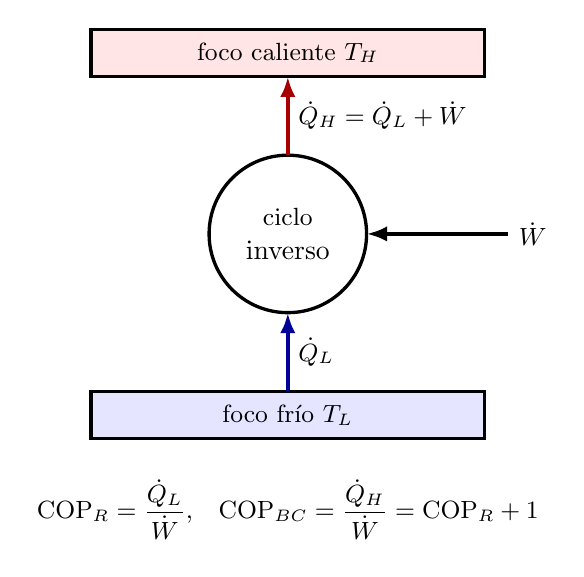
\begin{tikzpicture}[line width=1pt,>={Latex[length=2.6mm]}]
  % foco caliente (arriba)
  \fill[red!10] (0,3.6) rectangle (5,4.2); \draw[line width=1.1pt] (0,3.6) rectangle (5,4.2);
  \node at (2.5,3.9){\small foco caliente  $T_H$};
  % foco frio (abajo)
  \fill[blue!10] (0,-1.0) rectangle (5,-0.4); \draw[line width=1.1pt] (0,-1.0) rectangle (5,-0.4);
  \node at (2.5,-0.7){\small foco frío  $T_L$};
  % maquina (circulo central)
  \draw[line width=1.2pt] (2.5,1.6) circle (1.0);
  \node[align=center] at (2.5,1.6){\small ciclo\\inverso};
  % Q_L sube del foco frio a la maquina
  \draw[->,blue!60!black,line width=1.5pt] (2.5,-0.4)--(2.5,0.6); \node[right] at (2.5,0.1){\small $\dot Q_L$};
  % Q_H sube de la maquina al foco caliente
  \draw[->,red!65!black,line width=1.6pt] (2.5,2.6)--(2.5,3.6); \node[right] at (2.5,3.1){\small $\dot Q_H=\dot Q_L+\dot W$};
  % W entra
  \draw[->,black,line width=1.5pt] (5.3,1.6)--(3.5,1.6); \node[right] at (5.3,1.6){\small $\dot W$};
  % COP
  \node at (2.5,-1.9){\small $\mathrm{COP}_R=\dfrac{\dot Q_L}{\dot W}$,\quad $\mathrm{COP}_{BC}=\dfrac{\dot Q_H}{\dot W}=\mathrm{COP}_R+1$};
\end{tikzpicture}
\end{document}
